\documentclass[12pt]{article}



\usepackage{amsmath}
\usepackage{subfigure}
\usepackage{amssymb}
\usepackage{gregmath}
\usepackage{cite}
\usepackage{fancyhdr}
\usepackage{url}
\usepackage{color}
\usepackage{graphicx}
\usepackage[margin=1in]{geometry}

\graphicspath{{./pdf/}}


\begin{document}

\pagestyle{fancy}
\lhead{Gregory Ditzler}
\chead{\bfseries Rowan University}
\rhead{Advanced DSP}
\lfoot{\sf http://gregoryditzler.com}
\cfoot{  }
\rfoot{\today}
%\renewcommand{\headrulewidth}{0.4pt}
%\renewcommand{\footrulewidth}{0.4pt}


\begin{center}
  {\huge
    Introduction of Optimal Wiener Filters
  }
\end{center}




%\pagestyle{fancy}
%\lhead{Gregory Ditzler}
%\chead{\bfseries Rowan University}
%\rhead{Advanced Digital Signal Processing}
%\lfoot{\sf http://gregoryditzler.com}
%\cfoot{ \thepage }
%\rfoot{\today}






%%%%%%%%%%%%%%%%%%%%%%%%%%%%%%%%%%%%%%%%%%%%%%%%%%%%%%%%%%%%%%%
\section{Introduction \& Setup}
There are many setting where we have an input sequence $\{x[n]\}$ that consists of a desired input signal $\{s[n]\}$ which has been corrupted with undesirable additive noise $\{w[n]\}$. The goal, which is a fundamental principal in signal processing, is to filter the input signal such that the noise and interference is ameliorated from the output of the system responsible for filtering the signal. In todays lecture we shall treat the problem of filtering such a signal by estimating the presence of the additive noise. This estimation is constrained to a linear filter with an impulse response given by $\{h[n]\}$. The output of the filter produces the desired signal $\{d[n]\}$. Figure \ref{fig:lin est} shows the problem of this estimation using a linear filter. 

\begin{figure}[h!]
  \centering
  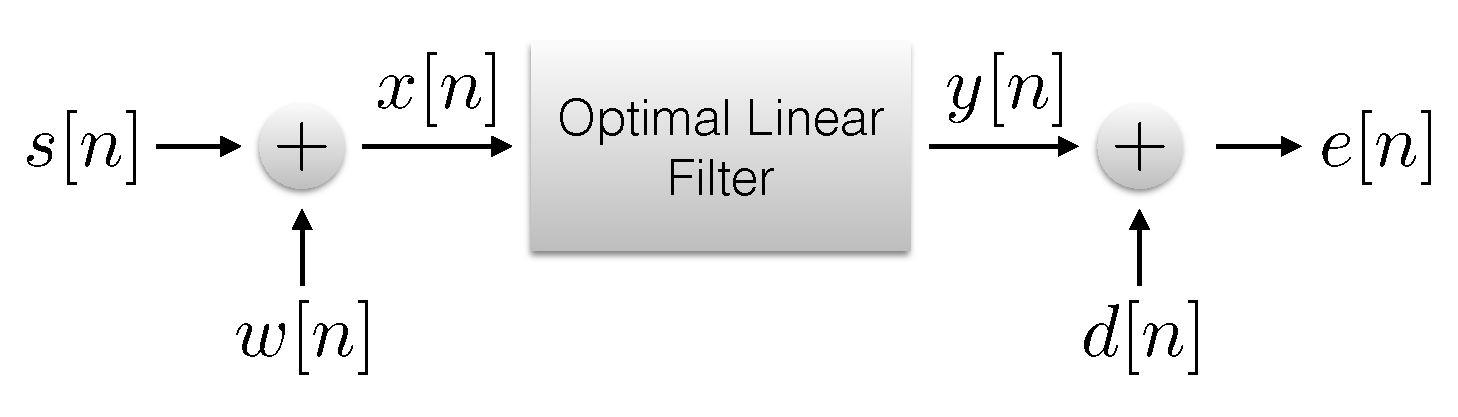
\includegraphics[width=.7\textwidth]{wiener.pdf}
  \caption{Model for a linear estimation problem. }
  \label{fig:lin est}
\end{figure}

The input signal $x[n] = s[n]+w[n]$ is presented to a linear filter with the output being given by $y[n]$. The error from this estimation is given by $e[n] = d[n] - y[n]$. There are three specific case to consider. 

\begin{itemize}
  \item If $d[n] = s[n]$ then the linear estimation problem is referred to as {\em filtering}. 
  \item If $d[n] = s[n+D]$, where $D > 0$ the problem is known as signal {\em prediction}. 
  \item If $d[n] = s[n-D]$, where $D > 0$ the problem is known as signal {\em smoothing}. 
\end{itemize}

In this lecture we focus on signal filtering and prediction. One of the central issues that we should make clear is that the user designing the filter must know the precise spectrum of the input domain to develop a precise filter. However, it is rarely the situation that the user is going to know all of these characteristics prior to building a filter. Often, we specify the filter characteristics based on some past experience, and/or trial and error. FIR/IIR design techniques can design any filter you specify -- it does not tell you whether that is the right filter for that specific signal. Our discussion of Wiener filters with present an approach to handling the situation where we do not have such prior knowledge. The {\em Wiener filter} is one such that it achieves the minimum mean-squared error (MMSE). 



%%%%%%%%%%%%%%%%%%%%%%%%%%%%%%%%%%%%%%%%%%%%%%%%%%%%%%%%%%%%%%%
\section{FIR Wiener Filters}


\begin{align}
  y[n] = \sum_{k=0}^{M-1} h[k] x[n-k]
\end{align}

\begin{align}
  \epsilon_M &= \Ebb\left[ |e[n]|^2 \right] \nonumber \\
  &= \Ebb\left[ \left| d[n] -  \sum_{k=0}^{M-1} h[k] x[n-k] \right|^2 \right]
\end{align}

\begin{align}
  \sum_{k=0}^{M-1} h[k] \gamma_{xx}[l-k] = \gamma_{dx}[l]
\end{align}

\begin{align}
  \boldsymbol{\Gamma}_M \hbf_{M} = \boldsymbol{\gamma}_d
\end{align}

\begin{align}
  \hbf_{\textrm{opt}} = \boldsymbol{\Gamma}_M^{-1} \boldsymbol{\gamma}_d
\end{align}

\begin{align}
  \textrm{MMSE}_{M} = \min_{\hbf_M} \epsilon_M &= \sigma_d^2 - \sum_{k=0}^{M-1}h_{\textrm{opt}}[k] \gamma_{dx}^*[k] \\
  &= \sigma_d^2 - {\boldsymbol{\gamma}_d^*}^{\T} \boldsymbol{\Gamma}_M^{-1} \boldsymbol{\gamma}_d
\end{align}

where $\sigma_d^2 = \Ebb[|d[n]|^2]$.

\end{document}

